\documentclass{boi2014-fi}

\usepackage{enumitem}
\usepackage{tikz}
\usepackage{todonotes}
\usepackage{wrapfig}

\renewcommand{\DayNum}{2}
\renewcommand{\TaskCode}{demarcation}
\renewcommand{\TaskName}{Rajanveto}

\newcommand{\constant}[1]{{\tt #1}}

\begin{document}
    \begin{wrapfigure}{r}{3cm}
        \vspace{-24pt}
        \includegraphics[width=3cm]{\TaskCode.jpeg}
    \end{wrapfigure}

    Byteotian saari oli pitkään oikeudenmukaisen kuninkaan Byteasarin vallassa.
    Mutta sitten kuningas kuoli ja hänen kaksi poikaansa --
    kaksoset Biteon ja Byteon -- eivät päässeet sopimukseen siitä,
    kumpi perisi kruunun.
    Sen vuoksi he päättivät jakaa saaren kahteen provinssiin
    ja hallita niitä riippumattomasti.

    Suorakulmion muotoisella kartalla Byteotiaa kuvaa monikulmio,
    jossa on $N$ kulmapistettä.
    Jokainen monikulmion sivu on samansuuntainen kuin kartan sivu,
    ja kaikki vierekkäiset sivut ovat suorassa kulmassa toisiinsa nähden.
    Biteon ja Byteon haluavat jakaa monikulmion kahdeksi yhteneväksi monikulmioksi
    yhdellä monikulmion sisään osuvalla janalla, joka on samansuuntainen
    kuin kartan sivu.
    (Kaksi kuviota ovat yhtenevät, jos ne voidaan muuttaa toisikseen
     yhdistelmällä peilauksia, kiertoja ja siirtoja.)
    Monikulmion kulmapisteiden koordinaatit sekä jakavan janan
    päätepisteiden koordinaatit ovat kokonaislukuja.

    Kuninkaan pojat antoivat tehtäväksesi tutkia,
    onko tällainen jako mahdollinen.

    \Task
    Annettuna on saaren muoto,
    ja tehtäväsi on määrittää, voidaanko se jakaa
    vaaka- tai pystysuunntaisella janalla kahdeksi yhteneväksi osaksi.
    Jos tämä on mahdollista, etsi yksi tällainen jana.
    
    \Input
    Syötteen ensimmäisellä rivillä on yksi kokonaisluku $N$,
    kulmapisteiden lukumäärä.
    Seuraavaksi tulee $N$ riviä, joista $i$:s sisältää kokonaisluvut
    $X_i$ ja $Y_i$, jotka ovat $i$:nnen kulmapisteen koordinaatit.
    Kulmapisteet annetaan järjestyksessä, eli
    janat $(X_1,Y_1) - (X_2,Y_2)$, $(X_2,Y_2) - (X_3,Y_3)$, \ldots, $(X_{N-1},Y_{N-1}) - (X_N,Y_N)$ sekä
    $(X_N,Y_N) - (X_1,Y_1)$ ovat kaikki monikulmion sivuja.


    \Output
    Ohjelmasi tulee tulostaa yksi rivi.
    Jos on mahdollista jakaa saari kahdeksi yhteneväksi osaksi
    vaaka- tai pystysuuntaisella janalla,
    jonka päätepisteet ovat $(x_1, y_1)$ ja $(x_2, y_2)$,
    tulosta 4 kokonaislukua $x_1$,
    $y_1$, $x_2$ ja $y_2$ välilyönnein erotettuina.
    Joko $x_1 = x_2$ tai $y_1 = y_2$ täytyy päteä.

    Jos sopivaa jakoa ei ole olemassa, tulosta yksi sana \constant{NO}.

    \clearpage

    \Examples
    \example
    {
        10 \newline
        0 0 \newline
        1 0 \newline
        1 1 \newline
        3 1 \newline
        3 5 \newline
        2 5 \newline
        2 3 \newline
        1 3 \newline
        1 2 \newline
        0 2
    }
    {
        1 2 3 2
    }
    {
        Huomaa, että tässä tilanteessa on useapi oikea ratkaisu.

        \begin{center}
            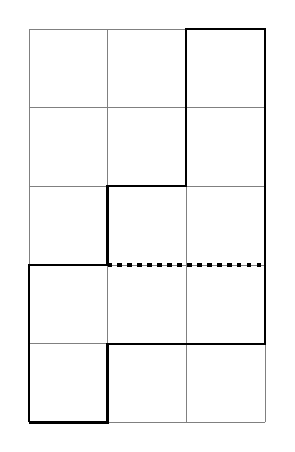
\begin{tikzpicture}
            \draw[help lines] (0,0) grid (3,5);
            \draw[thick] (0,0) -- (1,0) -- (1,1) -- (3,1) -- (3,5) --
                         (2,5) -- (2,3) -- (1,3) -- (1,2) -- (0,2) -- (0,0);
            \draw[ultra thick,dotted] (1,2) -- (3,2);
            \end{tikzpicture}
        \end{center}
    }

    \example
    {
        6 \newline
        0 0 \newline
        1 0 \newline
        1 1 \newline
        2 1 \newline
        2 2 \newline
        0 2
    }
    {
        NO
    }
    {
        Tässä tilanteessa ei ole tapaa jakaa saarta.
        \begin{center}
            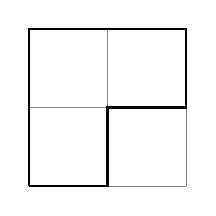
\begin{tikzpicture}
            \draw[help lines] (0,0) grid (2,2);
            \draw[thick] (0,0) -- (1,0) -- (1,1) --
                         (2,1) -- (2,2) -- (0,2) -- (0,0);
            \end{tikzpicture}
        \end{center}
    }

    \Scoring

    \begin{description}
        \item[Osatehtävä 1 (? pisteet).] $4 \le N \le 200$.
        \item[Osatehtävä 2 (? pisteet).] $4 \le N \le 4\ 000$.
        \item[Osatehtävä 3 (? pisteet).] $4 \le N \le 100\ 000$.
    \end{description}

    \Constraints

    \begin{description}
        \item[Aikaraja:] ? s.
        \item[Muistiraja:] ? MB.
    \end{description}

\end{document}
